% !TEX root = msc_thesis.tex

\begin{table}[tb]
	\caption[Datasets used for training, validating and testing core and interface predictors.]{Description of the datasets that were used in this study.}
	\label{tab:datasets}
	\begin{tabular}{ l |  p{1.8cm} | p{9.4cm} }
		\toprule
		Name                  & Type               & Description                                                                                                                                                                                                                                                                                                                  \\
		\midrule
		\textbf{Protherm}     & Train              & Mutation-induced changes in the Gibbs free energy of protein folding ($\Delta \Delta G_{core}$) compiled from the Protherm database \cite{bava_protherm_2004,kumar_protherm_2006} and from the datasets curated by Kellogg \textit{et al.} \cite{kellogg_role_2011}.                                                        \\
		\textbf{Skempi}       & Train              & Mutation-induced changes in the Gibbs free energy of protein-protein interaction ($\Delta \Delta G_{interface}$) compiled from the SKEMPI database \cite{moal_skempi:_2012} and the dataset curated by Kortemme and Baker \cite{kortemme_simple_2002}.                                                                      \\
		\textbf{Taipale}      & Validation         & Interaction between chaperones and wildtype or mutant proteins, quantified using the LUMIER assay \cite{sahni_widespread_2015}.                                                                                                                                                                                              \\
		\textbf{Taipale PPI}  & Validation         & Results of yeast two-hybrid experiments, measuring the presence or absence of protein-protein interactions for wild-type and mutant proteins \cite{sahni_widespread_2015}.                                                                                                                                                   \\
		\textbf{Taipale GPCA} & Validation         & \textit{Gaussia princeps} luciferase complementation assay, measuring the effect of mutations on protein affinity \cite{sahni_widespread_2015}.                                                                                                                                                                      \\
		\textbf{Humsavar}     & Validation \& Test & Disease-causing mutations and polymorphisms obtained from the UniProt \textit{humsavar.txt} file \cite{consortium_uniprot:_2015}. Mutations annotated with at least one disease are assigned a value of $1$. Mutations annotated as ``polymorphisms'' are assigned a value of $0$.                                         \\
		\textbf{ClinVar}      & Validation \& Test & Disease-causing mutations and polymorphisms obtained from ClinVar \cite{landrum_clinvar:_2016}. Mutations found in the ClinVar \textit{clinvar\-\_20160531.vcf} file are assigned a value of $1$. Mutations found in the ClinVar \textit{common\-\_no\-\_known\-\_medical\-\_impact\-\_20160531.vcf} file are assigned a value of $0$. \\
		\textbf{COSMIC}       & Validation \& Test & Mutations found in cancer \cite{forbes_cosmic:_2015}. Mutations classified by FATHMM \cite{shihab_ranking_2014} as cancer drivers are assigned a value of $1$. Mutations classified by FATHMM as cancer passengers are assigned a value of $0$.                                                                            \\
		\textbf{SUMO Ligase}  & Test               & Mutations affecting the activity of SUMO ligase, measured using a cell viability assay \cite{cagi4_sumo_ligase}.                                                                                                                                                                                                             \\
		\textbf{AB-Bind}      & Test               & Mutations explored in antibody-antigen affinity maturation experiments \cite{sirin_ab-bind:_2016}.                                                                                                                                                                                                                                   \\
		\textbf{Benedix}      & Test               & Results of alanine scanning experiments of the TEM1 ($\beta$-lactamase) -- BLIP ($\beta$-lactamase-inhibitor) interface \cite{benedix_predicting_2009}.                                                                                                                                                                              \\
		\bottomrule
	\end{tabular}
\end{table}

\clearpage

\begin{figure}[tb]
	\centering
	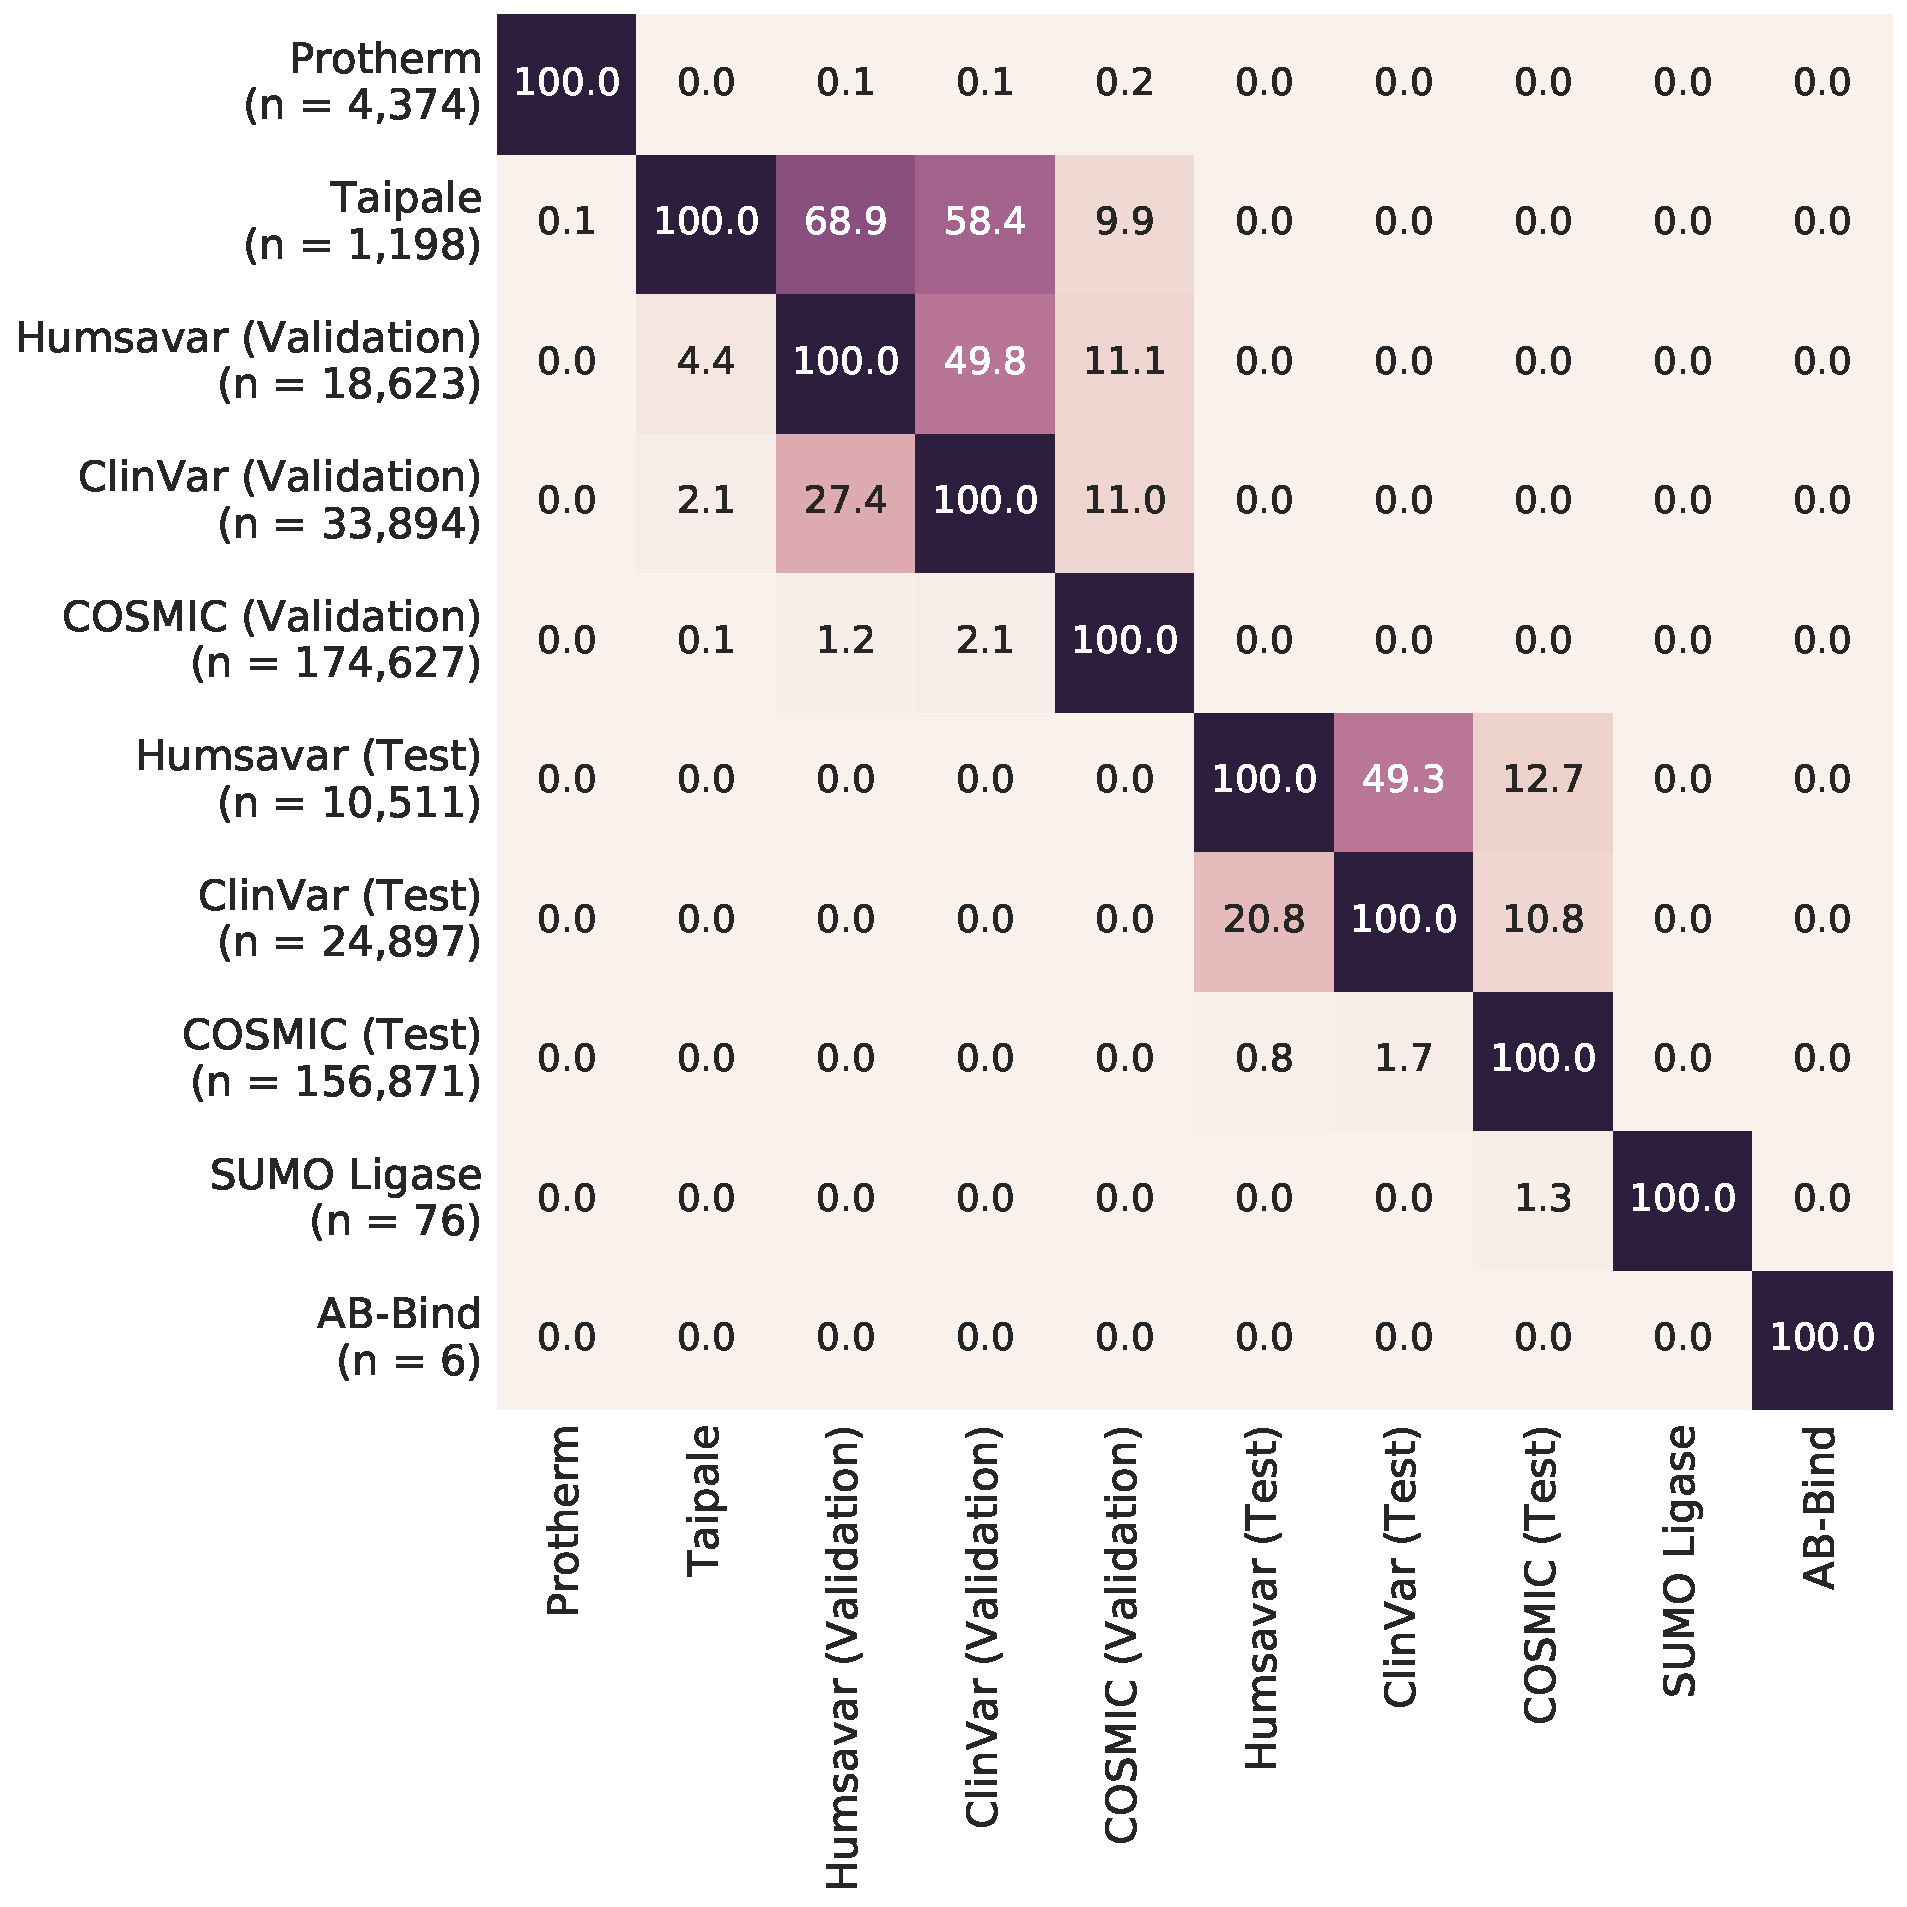
\includegraphics[width=0.8\textwidth]{static/elaspic_training_set/data_statistics/training_set_overlap_data_df_tt_core.pdf}
	\caption[Overlap in core mutation datasets.]{
		Overlap in core mutations between all the datasets used in this study.
		The shade and value inside each square denotes the percentage of mutations in the dataset named on the y-axis that are also found in the dataset named on the x-axis.
		Core mutations are defined as mutations that do not occur within 6 {\AA} of a neighbouring chain in the provided PDB structure or protein-protein homology model.
		A description of each dataset can be found in Table \ref{tab:datasets}.
	}
	\label{fig:training_set_overlap_core}
\end{figure}

\clearpage

\begin{figure}[tb]
	\centering
	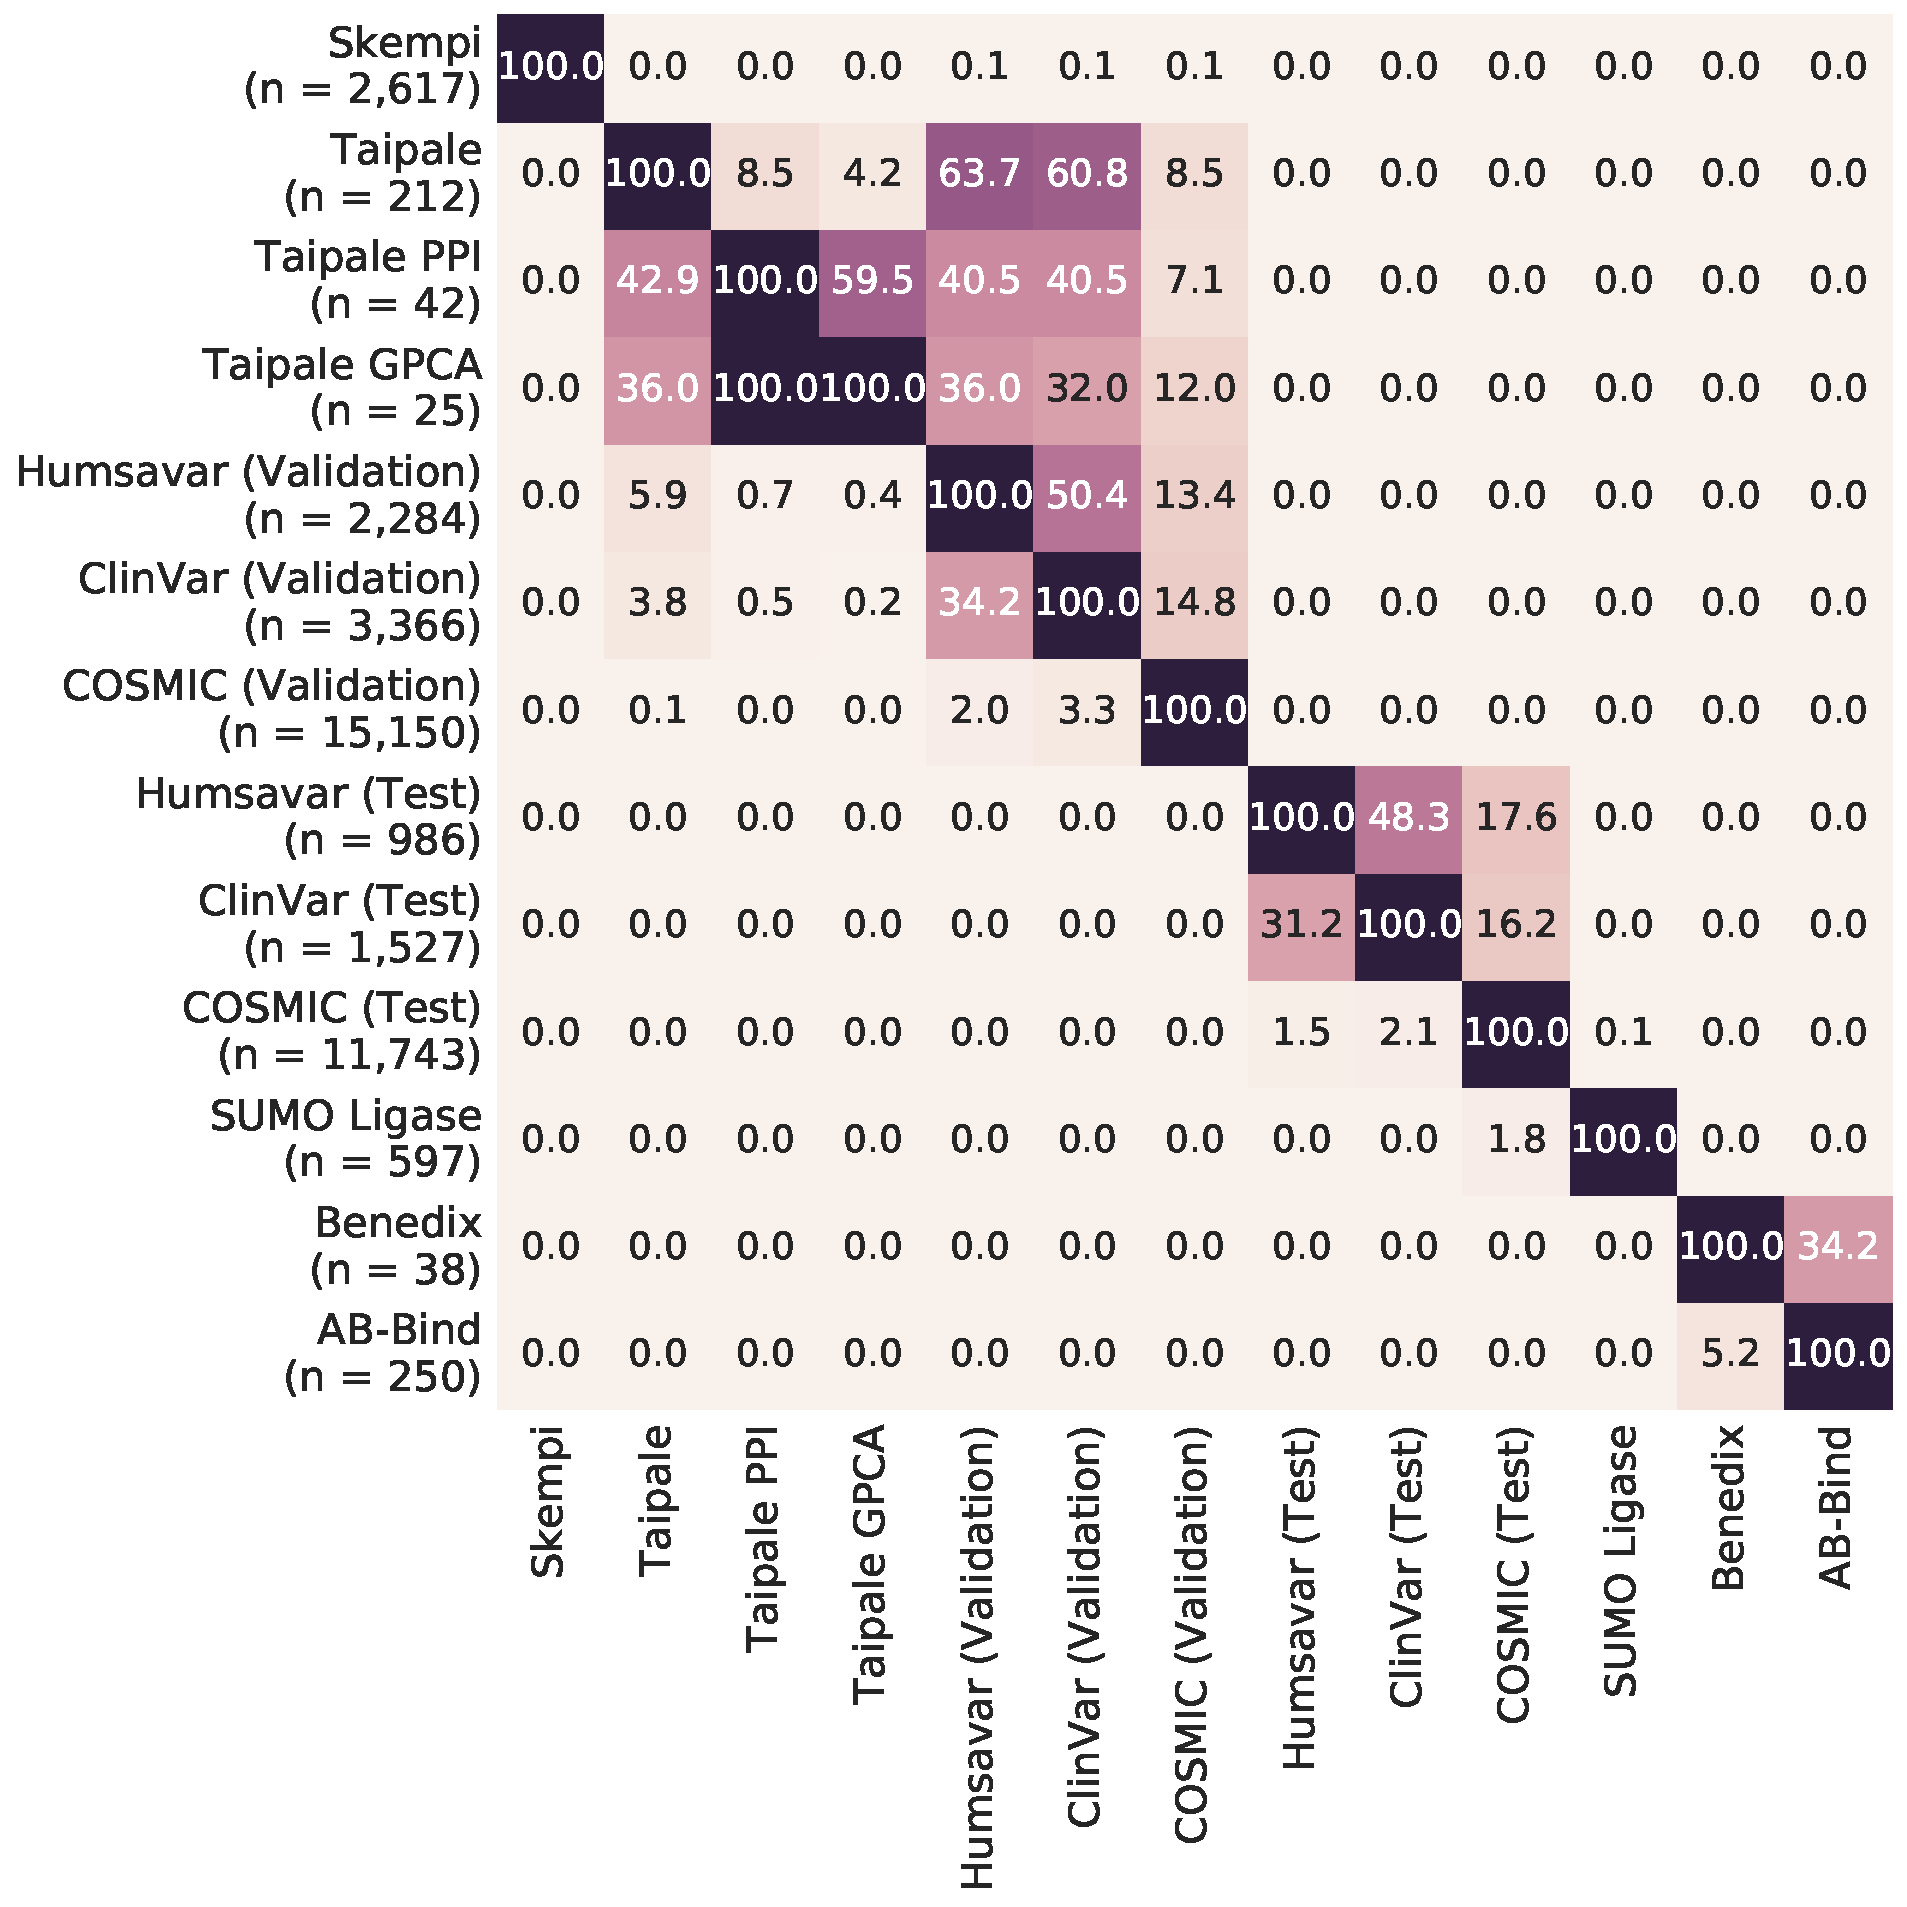
\includegraphics[width=0.9\textwidth]{static/elaspic_training_set/data_statistics/training_set_overlap_data_df_tt_interface.pdf}
	\caption[Overlap in interface mutation datasets.]{
		Overlap in interface mutations between all the datasets used in this study.
		The shade and value inside each square denotes the percentage of mutations in the dataset named on the y-axis that are also found in the dataset named on the x-axis.
		Interface mutations are defined as mutations that occur within 6 {\AA} of a neighbouring chain in the provided PDB structure or protein-protein homology model.
		A description of each dataset can be found in Table \ref{tab:datasets}.
	}
	\label{fig:training_set_overlap_interface}
\end{figure}
